% Preamble
\documentclass[11pt]{article}

% Packages
\usepackage{amsmath}
\usepackage{amssymb}
\usepackage{tikz}
\usetikzlibrary{arrows,arrows.meta,positioning,calc,petri}
\usepackage{adjustbox}
\usepackage{enumitem}
\usepackage{listings}
\usepackage[ruled,vlined]{algorithm2e}
\SetKwRepeat{Do}{do}{until}%
\newtheorem{theorem}{Theorem}

% Document
\begin{document}

    \section*{Rule~Q: Preemptive transition firing}
    Rule~Q evaluates transitions that are initially enabled and are the only consumer of all places in its pre set.
    The formal description of Rule~Q can be found in Figure~\ref{fig:rule_q}.
    Remark that Rule~Q can potentially put tokens into places which will prevent other reductions.
    Furthermore, it can be applied infinitely if $\boxminus(t_0)\leq \boxplus(t_0)$, or if the Petri net contains a loop.

    \begin{figure}[h!]
        \centering
        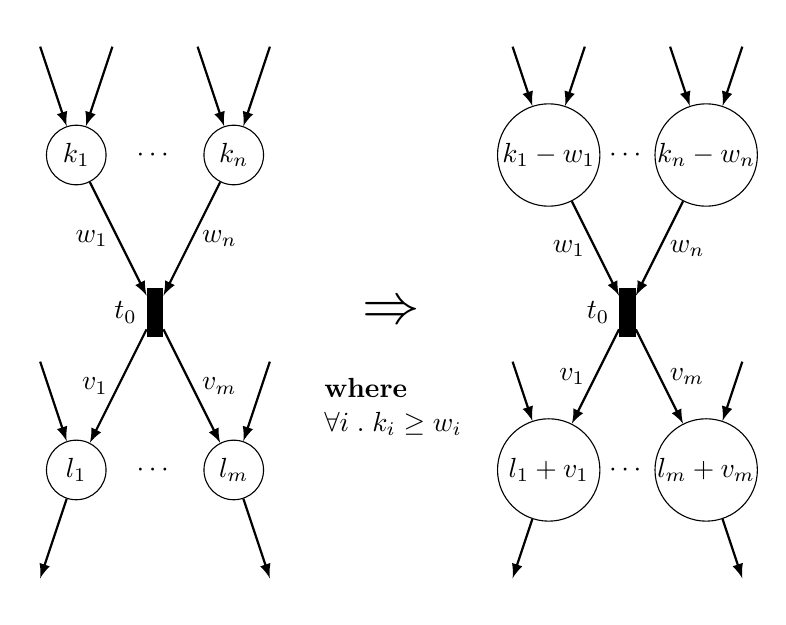
\begin{tikzpicture}
            % Left side places
            \node[place] (lplace1) at (0,2) {$k_1$};
            \node[place] (lplace2) at (2,2) {$k_n$};
            \node at (1,2) {$\cdots$};
            \node[place] (lplace3) at (0,-2) {$l_1$};
            \node[place] (lplace4) at (2,-2) {$l_m$};
            \node at (1,-2) {$\cdots$};

            % Left side transition
            \node[transition,minimum height=6mm,minimum width=2mm,fill=black,label=left:$t_0$] (ltrans) at (1,0) {};
            %\node[transition,minimum height=6mm,minimum width=2mm,fill=black,label=below:$t_0$] (remTrans1) at (0,-2) {};

            % Left side invisible nodes
            \node (lp1in1) at (-0.5,3.5) {};
            \node (lp1in2) at (0.5,3.5) {};
            \node (lp2in1) at (1.5,3.5) {};
            \node (lp2in2) at (2.5,3.5) {};
            \node (lp3in1) at (-0.5,-0.5) {};
            \node (lp4in1) at (2.5,-0.5) {};
            \node (lp3out1) at (-0.5,-3.5) {};
            \node (lp4out1) at (2.5,-3.5) {};

            % Left side arcs between transitions and nodes
            \draw[-latex,thick] (lplace1) edge node[left] {$w_1$} (ltrans);
            \draw[-latex,thick] (lplace2) edge node[right] {$w_n$} (ltrans);
            \draw[-latex,thick] (ltrans) edge node[left] {$v_1$} (lplace3);
            \draw[-latex,thick] (ltrans) edge node[right] {$v_m$} (lplace4);

            % Left side arcs to/from invisible nodes
            \draw[-latex,thick] (lp1in1) -- (lplace1);
            \draw[-latex,thick] (lp1in2) -- (lplace1);
            \draw[-latex,thick] (lp2in1) -- (lplace2);
            \draw[-latex,thick] (lp2in2) -- (lplace2);
            \draw[-latex,thick] (lp3in1) -- (lplace3);
            \draw[-latex,thick] (lp4in1) -- (lplace4);
            \draw[-latex,thick] (lplace3) -- (lp3out1);
            \draw[-latex,thick] (lplace4) -- (lp4out1);

            % ================== Middle arrow ==================
            \node (arrow) at (4,0) {\huge$\Rightarrow$};
            \node[text width=3.5cm] at (4.9, -1.2) {\textbf{where}\\$\forall i\;.\;k_i\geq w_i$};
            % ==================================================

            % Right side places
            \node[place,minimum size=1.3cm] (rplace1) at (6,2) {$k_1 - w_1$};
            \node at (7,2) {$\cdots$};
            \node[place,minimum size=1.3cm] (rplace2) at (8,2) {$k_n - w_n$};
            \node[place,minimum size=1.3cm] (rplace3) at (6,-2) {$l_1 + v_1$};
            \node at (7,-2) {$\cdots$};
            \node[place,minimum size=1.3cm] (rplace4) at (8,-2) {$l_m + v_m$};

            % Right side transition
            \node[transition,minimum height=6mm,minimum width=2mm,fill=black,label=left:$t_0$] (rtrans) at (7,0) {};
            %\node[transition,minimum height=6mm,minimum width=2mm,fill=black,label=below:$t_0$] (remTrans1) at (0,-2) {};

            % Right side invisible nodes
            \node (rp0in1) at (5.5,3.5) {};
            \node (rp0in2) at (6.5,3.5) {};
            \node (rp1in1) at (7.5,3.5) {};
            \node (rp1in2) at (8.5,3.5) {};
            \node (rp2in1) at (5.5,-0.5) {};
            \node (rp3in1) at (8.5,-0.5) {};
            \node (rp2out1) at (5.5,-3.5) {};
            \node (rp3out1) at (8.5,-3.5) {};

            % Right side arcs between transitions and nodes
            \draw[-latex,thick] (rplace1) edge node[left] {$w_1$} (rtrans);
            \draw[-latex,thick] (rplace2) edge node[right] {$w_n$} (rtrans);
            \draw[-latex,thick] (rtrans) edge node[left] {$v_1$} (rplace3);
            \draw[-latex,thick] (rtrans) edge node[right] {$v_m$} (rplace4);

            % Right side arcs to/from invisible nodes
            \draw[-latex,thick] (rp0in1) -- (rplace1);
            \draw[-latex,thick] (rp0in2) -- (rplace1);
            \draw[-latex,thick] (rp1in1) -- (rplace2);
            \draw[-latex,thick] (rp1in2) -- (rplace2);
            \draw[-latex,thick] (rp2in1) -- (rplace3);
            \draw[-latex,thick] (rp3in1) -- (rplace4);
            \draw[-latex,thick] (rplace3) -- (rp2out1);
            \draw[-latex,thick] (rplace4) -- (rp3out1);
        \end{tikzpicture}
        \vspace{1cm}

        \begin{adjustbox}{center}
            \begin{tabular}{|p{65mm}|p{45mm}|} \hline
            Precondition & Update \\ \hline
            Fix transition $t_0$ s.t.:
            \begin{itemize}[leftmargin=10mm]
                \item[Q1)] $({}^\bullet t)^\bullet = \{t_0\}$
                \item[Q2)] $\boxminus(t_0) \leq M_0 < I(t_0)$
                \item[Q3)] $({}^\bullet t_0 \cup t_0^\bullet) \cap
                places(\varphi) = \emptyset$
                \item[Q4)] $({}^\bullet t_0)^\circ = (t_0^\bullet)^\circ = \emptyset$
            \end{itemize}
            &
            \begin{itemize}[leftmargin=10mm]
                \item[UQ1)] $M_0:=M_0 + E(t_0)$.
            \end{itemize} \\ \hline
            \end{tabular}
        \end{adjustbox}
        \caption{Rule Q: Preemptive transition firing}
        \label{fig:rule_q}
    \end{figure}

    \begin{theorem}
        Rule~Q in Figure~\ref{fig:rule_q} is correct for CTL\textbackslash X.
    \end{theorem}

\end{document}
